\renewcommand{\lastmod}{3. Dezember 2024}
\renewcommand{\chapterauthors}{Markus Lippitz}

\chapter{Licht-Materie-Wechselwirkung}




% 6. Lasers
% Sim: Lasers
% • We originally covered Lasers towards the end of the course, but we realized that we didn’t
% actually use anything other than the basics of spectra in our treatment, and the engineers got
% grumpy if we spent too long on fundamentals without any applications, so we moved Lasers
% to so that there was more emphasis on applications early in the course. This worked much
% better.
% • When we ask students why laser beams are so powerful, it’s split 50/50 between more power
% in the beam and more concentrated light.
% • The homework on lasers starts with basic questions about absorption and spontaneous and
% stimulated emission, works through the steps of building a laser and troubleshooting a broken
% laser, and ends with essays on why a population inversion is necessary to build a laser and
% why this requires atoms with three energy levels instead of two. Most students are able to
% give coherent explanations in these es


\section{Überblick}
Die Spektroskopie atomarer Übergänge hat uns bereits in den ersten Kapiteln beschäftigt. Hier wollen wir sie etwas genauer betrachten und die Quantenmechanik nutzen, um \emph{Auswahlregeln} aufzustellen. Nicht zwischen allen Zuständen gibt es Übergänge, bei denen Licht absorbiert oder emittiert wird. Dies hängt mit der Symmetrie der Wellenfunktion und der Drehimpulserhaltung zusammen und wird im \emph{Übergangsdipolmonent} formalisiert.



Neben der 'gewöhnlichen' spontanen Emission gibt es den von A. Einstein postulierten Prozess der \emph{stimulierten Emission}. Einstein zeigte, dass sich ein Atom nur dann im thermischen Gleichgewicht mit dem umgebenden Strahlungsfeld befinden kann, wenn dieser Prozess existiert. Diese stimulierte Emission ist die Grundlage des Lasers. Dieser wurde 1960 zunächst als Effekt ohne wirkliche Anwendung demonstriert, ist aber aus der heutigen Technologie nicht mehr wegzudenken.

Schließlich betrachten wir noch einen ganz anderen Wellenlängenbereich: Die sehr kurzwellige Röntgenstrahlung entsteht ebenfalls durch atomare Übergänge, allerdings durch tief gebundene Elektronen und nicht durch Valenzelektronen wie beim sichtbaren Licht. Neben dem breiten \emph{Bremsspektrum} finden sich charakteristische Linien, die den atomaren Übergängen entsprechen. Dies wird im Moseley-Gesetz durch ein wasserstoffähnliches System modelliert, dessen Kernladung teilweise abgeschirmt ist.

Dieses Kapitel folgt \cite{Harris_moderne_Physik} mit großen Anteilen von \cite{Demtröder_ep3}.




\section{Dipol-Übergänge}

Bisher haben wir die Wellenfunktion eines Elektrons im Atom immer als $\Psi(\br)$ geschrieben, also nur eine Ortsabhängigkeit, aber keine Zeitabhängigkeit berücksichtigt. Es sind aber beschleunigte Ladungen, die elektromagnetische Wellen aussenden. Wir brauchen also auch die Zeitabhängigkeit der Wellenfunktion. Dies ist einfach für Wellenfunktionen, die zu einem Energieeigenwert $E$ gehören. In diesem Fall ist die Zeitkomponente einfach 
\begin{equation}
    \Psi(\br, t) = \Psi(\br) \, e^{- i \frac{E}{\hbar} \, t} \quad .
\end{equation}
Das ist wie bei einer ebenen Welle, die die Form 
\begin{equation}
    u(\br, t) = u_0 \, e^{i ( \bk \cdot \br - \omega t)}
\end{equation}
hat. Der räumliche Teil ist in $\Psi(\br)$ ausgelagert. Der zeitliche Teil ist identisch, da $E = \hbar \omega$.

Soll nun ein Atom von einem Zustand $\Psi_A$ in einen Zustand $\Psi_E$ übergehen, so ist es plausibel, dass es sich dabei zumindest für eine sehr kurze Zeit in einer Überlagerung der Form 
\begin{equation}
    \Psi_\text{Übergang} (\br, t) = \Psi_A(\br, t) + \Psi_E(\br, t) = 
    \Psi_A(\br) \, e^{-i E_A t / \hbar} +  \Psi_E(\br) \, e^{-i E_E t / \hbar}
\end{equation}
befindet. Da es hier nur um das Prinzip geht, werden alle Vorfaktoren und deren zeitliche Entwicklung\sidenote{Die Gewichtung zwischen Anfangs- und Endzustand sollte sich bei einem Übergang ja ändern.} weggelassen. Die Wahrscheinlichkeitsdichte ist dann
\begin{align}
    & \left| \Psi_\text{Übergang} (\br, t)  \right|^2 =  \Psi_\text{Übergang}^\star (\br, t) \Psi_\text{Übergang} (\br, t)  \\
   & =  \left(  \Psi_A^\star(\br) \, e^{+i E_A t / \hbar} +  \Psi_E^\star(\br) \, e^{+i E_E t / \hbar} \right)
    \left(  \Psi_A(\br) \, e^{-i E_A t / \hbar} +  \Psi_E(\br) \, e^{-i E_E t / \hbar} \right) \\
    & = | \Psi_A(\br)|^2 + | \Psi_E(\br)|^2  + 2 \Re \left\{ \Psi_A(\br)\Psi_E^\star(\br)  \, e^{-i (E_A - E_E) t / \hbar}  \right\}   \quad .
\end{align}
Wasserstoff-Wellenfunktionen sind reellwertig, so dass in der letzten Zeile auch das Konjugiert-Komplex weggelassen und die Exponentialfunktion durch einen Cosinus ersetzt werden kann.

Was passiert hier? Befindet sich ein Atom in einem Überlagerungszustand, so schwingt die Aufenthaltswahrscheinlichkeit des Elektrons und damit die Ladungsdichte mit der Kreisfrequenz $\omega_{AE} = (E_A - E_E) / \hbar $. Dies ist in Abbildung  \ref{fig:7_transition_panel} gezeigt. Die oszillierende Ladung sendet dann entweder elektromagnetische Wellen mit der Frequenz $\omega_{AE}$ aus oder wird, wie beim getriebenen Oszillator, von einer einfallenden elektromagnetischen Welle mit dieser Frequenz getrieben. Im ersten Fall wird Licht emittiert, im zweiten Fall absorbiert.

\begin{figure}    
    \inputtikz{\currfiledir transition_panel}
    \caption{ $| \eta \Psi_{1s} + \Psi_{2l} e^{i \omega t}|^2$ für $l= 0,1$. Nur im Fall $\Delta l = 1$ findet man eine oszillierende Ladungsverteilung. Hier ist $\eta < 1$ gewählt, um den Effekt besser sichtbar zu machen. Abbildung inspiriert von \cite{Reider_photonik}.}
    \label{fig:7_transition_panel}
\end{figure}


In der klassischen Elektronendynamik besteht ein Dipol aus einer positiven Ladung $q=+e$ am Ursprung und einer negativen Ladung $q=-e$ am Ort $\br$. Diese Ladungsverteilung hat das Dipolmoment $\bp = -e \br$. Für die Verteilung der Elektronen um einen positiven Kern im Ursprung integriert man über den Raum, d.h. 
\begin{equation}
    \bp = - \int_\text{Raum} e\br \,  | \Psi(\br, t) |^2 \, d \br   \quad .
\end{equation}
Die Wasserstoffwellenfunktionen sind alle punktsymmetrisch um den Ursprung. Daher tragen die Terme $ | \Psi_{A,E}(\br)|^2$ von $| \Psi_\text{Übergang}(\br,t)|^2$ nichts bei. Es bleibt 
\begin{equation}
    \bp =  - \Re \left \{ e^{-i (E_A - E_E) t / \hbar}  \, \int_\text{Raum} e\br \,  \Psi_A(\br)\Psi_E^\star(\br)  \, d \br \right \} \quad .
\end{equation}
Das räumliche Integral bestimmt vollständig, wie gut der Übergang $A \rightarrow E$ mit Licht möglich ist. Man nennt diesen Term \emph{Übergangs-Dipolmoment} oder Dipol-Matrixelement $\bM_{EA}$.
\begin{equation}
    \bM_{EA} = \int_\text{Raum} e\br \,  \Psi_A(\br)\Psi_E^\star(\br)  \, d \br  \quad .
    \label{eq:7_Matrix_element}
\end{equation}
Es handelt sich um einen Vektor, da das Integral als gewichtete Summe der Vektoren $\br$ aufgefasst werden kann.




\section{Auswahlregeln für Dipolübergänge}

In den meisten Fällen ist der genaue Wert des Übergangs-Dipolmoments $\bM_{EA}$ nicht von Bedeutung. Von Interesse ist vielmehr, ob für eine gegebene Kombination der Zustände $A$ und $E$ sein Betrag $|\bM_{EA}|$ von Null verschieden ist oder nicht. Ist er ungleich Null, so wird dieser Übergang als erlaubt bezeichnet, andernfalls als verboten. 

Wir suchen nun nach Regeln, die diese erlaubten Übergänge identifizieren. Dies sind die Auswahlregeln. Tatsächlich ist $|\bM_{EA}|$ für die meisten Kombinationen gleich Null. Das liegt an der Symmetrie der Wellenfunktionen. Wäre $\br$ nicht im Integral, dann wäre das Integral für alle $A \neq E$ Null, da die Wellenfunktionen orthonormiert sind.

Sehr viel erreicht man schon bei der Betrachtung der  \emph{Parität}. Die Parität einer Funktion $f$ beschreibt, wie sie sich unter Spiegelung aller Koordinaten verhält. Man bezeichnet sie als gerade oder ungerade, je nachdem ob das $n$ in 
\begin{equation}
    f(\br) = (-1)^n f(- \br)
\end{equation}
gerade oder ungerade ist. Bei gerader Parität ist also $f(\br) = + f(- \br) $.
Eine Funktion kann auch keine Parität haben, z. B. $f(x) = 1 + x$. Für Wasserstoffwellenfunktionen ist die Parität $(-1)^l$, d.h. gerade für gerade $l$. Das $\br$ in Gl. \ref{eq:7_Matrix_element} hat eine ungerade Parität und das Integral verschwindet, wenn die Parität insgesamt ungerade ist. Daher muss sich die Parität von $\Psi_A$ von der Parität von $\Psi_B$ unterscheiden, d.h. sie muss sich beim Übergang ändern. Dies ist die erste Auswahlregel, die immer gültig ist.

Der Spin in den Zuständen $A$ und $E$ ist ortsunabhängig. Der Spinanteil der Wellenfunktionen\sidenote{den wir bisher nie explizit geschrieben haben} kann also vor das Integral gezogen werden. Da auch die Spin-Wellenfunktionen orthonormal sind, kann sich der (Gesamt-)Spin bei einem Übergang nicht ändern. Allerdings gibt es die Spin-Bahn-Kopplung. Diese führt zu einem Einfluss des Spins auf den räumlichen Teil der Wellenfunktion, so dass nicht mehr alles vor das Integral gezogen werden kann. Die Spin-Erhaltung gilt also nicht strikt und immer weniger, je mehr die Spin-Bahn-Kopplung mit steigender Kernladung zunimmt.

\newpage

Hier nun ein Überblick über die Auswahlregeln
\begin{description}\setlength{\itemsep}{0pt}
    \item[Es gilt immer] \ \\
\begin{itemize}\setlength{\itemsep}{0pt}
    \item Die Parität muss sich ändern.
    \item $\Delta J = 0, \pm 1$, aber der Übergang $J=0$ nach $J=0$ ist verboten.
    \item $\Delta m_J = 0, \pm 1$, aber der Übergang $m_J=0$ nach $m_J=0$ ist verboten, falls $\Delta J = 0$.
\end{itemize}

\item[Für Einelektron-Atome]  gilt immer  \ \\
\begin{itemize}\setlength{\itemsep}{0pt}
    \item  $\Delta l = \pm 1$ (aber  $\Delta l = 0$ ist verboten)
    \item $\Delta s = 0$, weil ein Elektron immer $s=1/2$ besitzt.
\end{itemize}

\item[Für Mehrelektron-Atome] gilt im Bereich der LS-Kopplung   \ \\  
\begin{itemize}\setlength{\itemsep}{0pt}
    \item $\Delta S = 0$, gilt durch die LS-Kopplung aber nur schwach.
    \item $\Delta L = \pm 1$. In Spezialfällen (mehr als ein Elektron verändert seine Wellenfunktion) ist auch $\Delta L = 0$ erlaubt. Dann ist immer noch der Übergang $L=0$ nach $L=0$  verboten.
\end{itemize}

\item[Für schwerere Mehrelektron-Atome]  jenseits  der LS-Kopplung gibt es \emph{zusätzlich} zu den Übergängen der LS-Kopplung noch mit geringerer Wahrscheinlichkeit    
\begin{itemize}\setlength{\itemsep}{0pt}
    \item $\Delta S  = \pm 1$
    \item $\Delta L =  \pm 2$ 
\end{itemize}
\end{description}

Es gibt keine Auswahlregel, die eine Änderung der Hauptquantenzahl $n$ verlangt! Insbesondere bei schweren Atomen sind die Energien zwischen den Zuständen gleicher Hauptquantenzahl so verschieden, dass relevante optische Übergänge auftreten, wie wir unten am Beispiel von Natrium sehen werden.

\subsection{Drehimpuls und Polarisation}

Neben Parität und Spin ist es die Drehimpulserhaltung, die die Auswahlregeln bestimmt.
Die Drehimpulserhaltung wird bei optischen Übergängen nicht verletzt, da auch das Photon einen intrinsischen Drehimpuls, den Spin $\bS_\gamma$, besitzt. Wir haben bereits in Tabelle \ref{tab:6_bosonen_fermionen} gesehen, dass dieser Spin 1 ist, also ganzzahlig, und dass Photonen daher Bosonen sind. Es gibt auch eine Orientierungsquantenzahl $m_\gamma$. Die Orientierungsquantenzahl kann für Photonen nur die Werte $m_\gamma = \pm 1$ annehmen. Diese entsprechen links- bzw. rechts zirkular polarisiertem Licht, oft auch als $\sigma^+$ bzw. $\sigma^-$ Licht bezeichnet. Eine elektromagnetische Welle hat eine eingebaute Vorzugsrichtung, die Richtung des Wellenvektors $\bk$. Entlang dieser Richtung wird daher die quantisierte Komponente $m_\gamma$ des Drehimpulses angegeben. Den Fall $m_\gamma = 0$ gibt es nicht, da Licht eine Transversalwelle ist. Zirkulare Polarisationen sind die Eigenzustände von Photonen. Linear polarisiertes Licht ist eine Überlagerung der beiden zirkularen Polarisationen.

Es muss also insgesamt die Drehimpulserhaltung gelten:
\begin{align}
    \bJ_A = \bJ_E + \bS_\gamma  & \quad \text{Emission} \\
    \bJ_A + \bS_\gamma = \bJ_E & \quad \text{Absorption} \quad .
\end{align}
Bleiben wir der Einfachheit halber bei den Absorptionsvorgängen. Für die Quantenzahl $J_E$ des Drehimpulses $\bJ_E$ am Ende des Prozesses gilt aus der Drehimpulsaddition
\begin{equation}
    | J_A - S_\gamma | \le J_e \le J_A - S_\gamma
\end{equation}
mit $S_\gamma = 1$. Dies beschreibt also $\Delta J = 0, \pm 1$. Die Orientierungsquantenzahl ist einfach die Summe
\begin{equation}
    m_{J,A} + m_\gamma = m_{J,E} \quad .
\end{equation} 
$\Delta m_J = \pm 1$ entspricht also $ m_\gamma = \pm 1$ bei Absorption (bei Emission ändert sich das Vorzeichen). Diese Übergänge sind also selektiv für die jeweiligen zirkularen Polarisationen. Der Übergang $\Delta m_J = 0$ erfordert linear polarisiertes Licht, also eine Überlagerung der beiden zirkularen Polarisationen.


Für das Ein-Elektronen-Atom lässt die Drehimpulserhaltung eigentlich auch $\Delta l = 0$ zu. Dieser Fall ist jedoch verboten, da sich die Parität bei $\Delta l = 0$ nicht ändert. Übergänge in Mehrelektronenatome sind sehr häufig von der Art, dass nur ein Elektron seine Quantenzahl ändert. In diesem Fall sind die Auswahlregeln im Grunde die gleichen wie für das Ein-Elektronen-Atom. Nur in seltenen Fällen führt die Absorption eines Photons zu einer Änderung bei zwei Elektronen. Diese Übergänge können dann auch $\Delta L = 0$ zeigen.



\subsection{Höhere Ordnungen}


Neben den oben besprochenen elektrischen Dipolübergängen gibt es auch magnetische Dipolübergänge, die also einem oszillierenden magnetischen Dipol entsprechen, und alle anderen Multipole, also Quadrupole, Oktupole usw. Diese Übergänge sind in der Regel schwächer und haben andere Auswahlregeln. Unter bestimmten Bedingungen kann ein Photon auch eine Art Bahndrehimpuls besitzen. Die elektromagnetische Welle ist dann keine ebene Welle mehr. Solche Photonen führen dann zu  anderen Auswahlregeln.



\section{Beispiel: Helium}

\begin{marginfigure}
    \inputtikz{\currfiledir helium} 
    \caption{Termschema von Helium mit einigen erlaubten Übergängen. Man erkennt die Aufspaltung nach dem Gesamtspin. Grau strichliert die Wasserstoff-Niveaus zum Vergleich. Der 1S-Zustand ist verschoben. Die J-Aufspaltung ist vergrößert.}
    \label{fig:7_helium}
\end{marginfigure}

Abbildung \ref{fig:7_helium} zeigt die niedrigsten Zustände von Helium. Diese wurden bereits am Ende des letzten Kapitels besprochen. Die grauen Linien zeigen  zulässige Übergänge. Zunächst fällt auf, dass die Übergänge innerhalb ihrer Multiplizität bleiben. Es gibt keinen erlaubten Übergang vom Singulett zum Triplett und umgekehrt, was eine Folge der Regel $\Delta S = 0$ ist. Dann ändern alle Übergänge die 'Spalte' im Diagramm, d.h. $\Delta L = \pm 1$. Bei Helium wird in diesen Zuständen nur ein Elektron angeregt. Der Sonderfall $\Delta L = 0$ tritt daher nicht auf. Es gibt zwei metastabile Zustände, $2^1S_0$ und $2^3S_1$, die keinen erlaubten Zerfallskanal besitzen. Die Spin-Bahn-Kopplung und Wechselwirkungen jenseits der hier beschriebenen Dipolstrahlung führen aber auch diese Zustände wieder in den Grundzustand zurück.



\section{Beispiel: Natrium}

\begin{marginfigure}
    \inputtikz{\currfiledir natrium} 
    \caption{Termschema von Natrium mit einigen erlaubten Übergängen. Rot sind die beiden gelben D-Linien. Grau strichliert die Wasserstoff-Niveaus zum Vergleich.}
    \label{fig:7_natrium}
\end{marginfigure}

Natrium ähnelt Wasserstoff in dem Sinne, dass ein einziges Valenzelektron seine Eigenschaften bestimmt. Die Elektronenkonfiguration ist [Ne]3s$^1$. Abbildung  \ref{fig:7_natrium} zeigt die niedrigsten angeregten Zustände und die Übergänge zwischen ihnen. Der Grundzustand hat das Termsymbol 3$^2$S$_{1/2}$, also ein Doublet. Charakteristisch sind die \emph{Natrium-D-Linien} bei 589,5 nm bzw. 588,9 nm Wellenlänge, die z.B. im gelben Licht einiger Straßenlaternen zu sehen sind.
Dies sind Übergänge aus den Zuständen 3$^2$P$_{1/2}$ und 3$^2$P$_{3/2}$. Dabei ist $\Delta S = 0$, $\Delta L = 1$ und $\Delta J = 0$ bzw. $1$. Die Hauptquantenzahl $n$ ändert sich also nicht. Die Feinstrukturaufspaltung $J = 1/2$ und $J=3/2$ führt zum Doublett der Linien.

\section{Lebensdauer angeregter Zustände}

Nachdem ein Atom durch die Absorption eines Photons oder durch einen Stoß in einen angeregten Zustand versetzt wurde, fällt es früher oder später wieder in den Grundzustand zurück. Dabei gibt es zwei Zeitspannen: Die Lebensdauer des angeregten Zustandes, also die Zeit, die das Atom in diesem Zustand bleibt, bevor es wieder zurückfällt, und die Dauer des Quantensprungs selbst. Der Quantensprung ist instantan. Das Atom verbringt also keine Zeit im Übergang selbst. Die Zeit bis zum Übergang lässt sich aber leicht messen: Man regt ein Gas von Atomen mit einem kurzen Lichtblitz an und misst die Helligkeit des abgestrahlten Lichts als Funktion der Zeit. Man findet einen exponentiellen Zerfall mit einer Zeitkonstante von typischerweise etwa 10~ns.

Was bedeutet das? Die Wahrscheinlichkeit, dass ein gegebenes angeregtes Atom ein Photon emittiert, ist unabhängig vom zeitlichen Abstand $t$ zwischen Anregungspuls und Detektionszeitfenster. Wie beim Würfeln ist die Wahrscheinlichkeit, eine Sechs zu würfeln, unabhängig von der Anzahl der bisherigen Würfe. Je öfter man würfelt, desto wahrscheinlicher ist es, dass es einmal passiert. Für jedes einzelne betrachtete Atom kann man also nicht sagen, wann es das Photon aussenden wird. Für alle Atome zusammen kann man jedoch die Anzahl $N$ der Atome in angeregten Zuständen angeben, und diese Anzahl nimmt mit einem Exponentialgesetz ab: 
\begin{equation}
    \frac{d N}{dt} = - \frac{N}{\tau}  = -k \, N \quad \text{und also} \quad N(t) =  N_0 \, e^{- t / \tau}  = N_0 \, e^{- k \, t }  \quad .
\end{equation} 
Dabei nennt man $\tau$ die Lebensdauer des angeregten Zustands und $k = 1 / \tau$ die Zerfallsrate.


\section{Einstein-Koeffizienten}



Im Jahre 1917, also noch vor dem Bohrschen Atommodell und der de Broglie-Wellenlänge, erkannte A.~Einstein, dass es neben den oben besprochenen Absorptions- und Emissionsprozessen noch einen weiteren Prozess geben muss, damit ein Atom im thermischen Gleichgewicht mit dem umgebenden (Schwarzkörper-) Licht sein kann. Betrachten wir dazu noch einmal Absorption und Emission.

Wir vereinfachen das Atom auf zwei Niveaus mit den Besetzungen $N_1$ und $N_2$. Die oben beschriebene Emission nennen wir \emph{spontane Emission}, da sie ohne äußere Einwirkung erfolgt. Die Übergangsrate $A_{21}$ nennt sich \emph{Einsteinkoeffizient der spontanen Emission}:
\begin{equation}
    \frac{d N_2}{dt} = - A_{21} \, N_2  \quad \text{spontane Emission} \quad . \label{eq:7_k_spontan}
\end{equation}


Damit eine Absorption stattfinden kann, das Atom also vom Zustand 1 in den Zustand 2 übergehen kann, muss ein Lichtfeld vorhanden sein. Dieses Feld habe die spektrale Energiedichte $u(E)$. Die Übergangsrate ist dann
\begin{equation}
    \frac{d N_1}{dt} = - B_{12} \, N_1 \, u(E_2 - E_1) \quad \text{Absorption} \label{eq:7_k_abs}
\end{equation}
$B_{12}$ ist der \emph{Einstein-Koeffizient der Absorption}.


\begin{marginfigure}
    \inputtikz{\currfiledir einstein-coeff}
    \caption{Die drei Einstein-Koeffizienten.}
\end{marginfigure}

Im thermodynamischen Gleichgewicht muss die Besetzung $N_i$ der Zustände über die Zeit konstant sein und das Verhältnis $N_2 / N_1$ muss der Boltzmann-Statistik entsprechen. Dies kann nur erreicht werden, wenn es auch den  Prozess der stimulierten Emission gibt. Dabei stimuliert  (oder induziert) ein einfallendes Photon den Zerfall eines angeregten Atoms, inklusive der Emission eines weiteren Photons. Vorher gibt es ein Photon udn ein Atom im angeregten Zustand, nachher  zwei Photonen und ein Atom im Grundzustand. Das zweite Photon ist dabei eine exakte Kopie des ersten. Die Übergangsrate ist $B_{21}$, der  \emph{Einstein-Koeffizienten der stimulierten Emission}:
\begin{equation}
    \frac{d N_2}{dt} = - B_{21} \, N_2 \, u(E_2 - E_1)  \quad \text{stimulierte Emission}  \quad .\label{eq:7_k_stim}
\end{equation}


Im thermischen Gleichgewicht muss die Rate aus Zustand 1 heraus  der Summe der Raten aus Zustand 2 heraus entsprechen, 
oder 
\begin{equation}
    B_{12} \, N_1 \, u(E_2 - E_1) =   A_{21} \, N_2 + B_{21} \, N_2 \, u(E_2 - E_1)  \quad .
\end{equation}
Und das Verhältnis der Besetzung muss der Boltzmann-Verteilung gehorchen
\begin{equation}
    \frac{N_2}{N_1} = \frac{g_2}{g_1} \, e^{- h \nu / (k_B T)}
\end{equation}
mit $h \nu = E_2 - E_1$ und $g_i = 2J +1$ der Entartung des Zustands $i$. Mit der spektralen Energiedichte des Schwarzkörpers (siehe Kapitel 2)
\begin{equation}
    u(\nu) = \frac{8 \pi h \nu^3}{c^3} \,  \frac{1}{e^{h\nu/k_B T} -1}
\end{equation}
findet man folgende Zusammenhänge zwischen den drei Einstein-Koeffizienten
\begin{equation}
   g_1 B_{12}  = g_2 B_{21} \quad \text{und} \quad
   A_{21} = \frac{8 \pi h \nu^3}{c^3}\, B_{21}  \quad. 
\end{equation}
Es gibt also nur einen freien Parameter, der direkt mit dem Übergangsdipolmoment $|\bM_{21}|^2$ zusammenhängt.


\section{Der Laser}
%\phet{Lasers}

Stimulierte Emission spielt unter normalen Bedingungen praktisch keine Rolle. Ein Atom befindet sich nur für sehr kurze Zeit im angeregten Zustand. Genau in diesem Moment müsste ein geeignetes stimulierendes Photon vorhanden sein. Das ist selten. Oder umgekehrt: In den allermeisten Situationen ist die stimulierte Rate viel kleiner als die spontane, also 
\begin{equation}
    u(h\nu)  B_{21}  \ll A_{21} = \frac{8 \pi h \nu^3}{c^3} \, B_{21} 
\end{equation}
weil 
\begin{equation} 
    \frac{1}{e^{h\nu/k_B T} -1} \ll 1 \quad .
\end{equation}

Niemand zweifelte an der von Einstein eingeführten stimulierten Emission, aber es dauerte bis in die 1950er Jahre, bis sie sinnvoll genutzt wurde. 1960 demonstrierte Theodore Maiman den ersten 'Laser'. Die Abkürzung steht für 'light amplification by stimulated emission of radiation' (Lichtverstärkung durch stimulierte Emission von Strahlung). Das Konzept geht zurück auf den von Charles H. Townes\sidenote{dafür Nobelpreis 1963} 1954 demonstrierten 'Maser' (microwave amplification by...). Die theoretische Beschreibung geht auf Arthur L. Schawlow\sidenote{Nobelpreis 1981 für Laserspektroskopie} zurück.

Die stimulierte Emission sollte also der dominierende Prozess sein, wenn ein Photon mit einem Atom wechselwirkt. Wenn wir aber der Einfachheit halber die Entartung gleichsetzen ($g_1 = g_2$), dann muss wegen der Ähnlichkeit von Gl. \ref{eq:7_k_abs} und \ref{eq:7_k_stim} die Besetzung im oberen Zustand größer sein als die im unteren Zustand, im Idealfall viel größer: $N_2 \gg N_1$. Andernfalls würde ein einfallendes Photon einfach absorbiert und nicht durch stimulierte Emission kopiert. Der Fall $N_2 > N_1$ wird als \emph{Besetzungsinversion} bezeichnet. Er ist nicht im thermischen Gleichgewicht. Für keine Temperatur $T$ liefert die Boltzmannverteilung eine solche Besetzung.

Wie erreichen wir die Besetzungsinversion? Wir müssen den Atomen Energie zuführen. Wir nehmen hier einmal an, dass dies durch Licht geeigneter Wellenlänge geschieht. Das nennt man \emph{optisches Pumpen}. So hat es Maiman in seinem Rubin-Laser gemacht. Heute kann man die Energie auch anders zuführen, zum Beispiel elektrisch. Es hilft nicht, wenn das Pumplicht den Übergang $1 \rightarrow 2$ pumpt. Zunächst nimmt zwar die Besetzung des Zustands 1 mit steigender Pumpintensität zu. Wenn wir aber die Gleichbesetzung erreichen ($N_1 = N_2$), dann wird ein einfallendes Pumpphoton mit der gleichen Wahrscheinlichkeit absorbiert, wie es stimulierte Emission verursacht. Diese Grenze kann nicht überschritten werden, und $N_2 > N_1$ wird nie erreicht.


\begin{marginfigure}
   \inputtikz{\currfiledir laser_levels_234}
    \caption{Laser mit 3 oder 4 Niveaus. Ein 2-Niveau-Laser kann nicht optisch gepumpt werden.}
    \label{fig:7_laser_niveau_34}
\end{marginfigure}

Der Ausweg ist ein System, das aus mehr als zwei Niveaus besteht, z.B. drei oder vier (siehe Abbildung  \ref{fig:7_laser_niveau_34}). Wir pumpen den Übergang $1 \rightarrow 3$. Der Zustand 3 ist kurzlebig und geht schnell in den Zustand 2 über, möglicherweise unter Aussendung eines Photons, das uns hier nicht interessiert. Damit ist die Besetzung $N_3 \ll N_1$ zu jedem Zeitpunkt, so dass dieser Übergang gut gepumpt werden kann. Gleichzeitig können wir  Besetzung im Zustand 2 akkumulieren und so $N_2 > N_1$ erreichen.

\begin{marginfigure}
    \inputtikz{\currfiledir laser_design}
    \caption{Ein Laser besteht aus Pump-Quelle, aktivem Medium und zwei Spiegeln als Resonator.}
    \label{fig:7_laser_design}
\end{marginfigure}


Neben der Energiequelle zum Pumpen und dem atomaren Gas als Verstärkungsmedium benötigt man einen Resonator, d.h. zwei Spiegel, die das Verstärkungsmedium umschließen. Die stimulierte Emission findet nicht bei jedem Durchgang eines Photons durch das Medium statt.  Der Resonator sorgt dafür, dass jedes Photon viele Chancen hat, einmal kopiert zu werden. Ist dies einmal geschehen, entsteht eine Art Lawine identischer Photonen, bis die stimulierte Emission ausreicht, um die Besetzungsinversion abzubauen und den Zustand $N_2 = N_1$ zu erreichen. Der Laser ist also eine Quelle identischer Photonen. Dies entspricht klassischerweise kohärentem Licht.


\section{Beispiel: Rubin-Laser}

Der historisch erste Laser verwendet Rubin als aktives Medium. Rubin ist ein Korund-Mineral, Chromaluminiumoxid, d.h. Chrom-Ionen in einer Aluminiumoxidmatrix (\ch{Al2O3}). Aluminiumoxid ist durchsichtig wie Glas. Ein Stab aus diesem Material ist an den Enden poliert und verspiegelt. Chrom ist in sehr geringer Menge (0,05\%) eingelagert. Die \ch{Cr^{3+}}-Ionen werden durch eine Blitzlampe in hoch angeregte Zustände gepumpt. Von dort zerfallen sie in einen tieferliegenden angeregten Zustand. Die überschüssige Energie wird in Form von Wärme an den Stab abgegeben. Der Rubinlaser ist somit ein Festkörperlaser und arbeitet bei einer Wellenlänge von 694.3~nm, an der Grenze zum nahen Infrarot. 

\begin{marginfigure}
    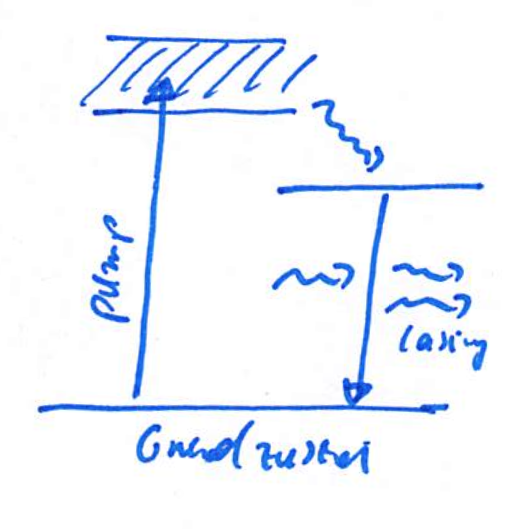
\includegraphics[width=\textwidth]{\currfiledir png/ruby.png}
    \caption{Die relevanten Zustände des Rubin-Lasers.}
    \label{fig:7_ruby_laser}
\end{marginfigure}

\section{Helium-Neon-Laser}

Der \ch{He:Ne}-Laser verwendet Neon als aktives Medium und Helium zur Anregung in einer Gasentladungsröhre. Die beschleunigten Elektronen regen das Helium durch Stöße vom Zustand 1s$^2$ in den Zustand 1s~2s an. Dieser Zustand kann wegen der Auswahlregel $\Delta l = \pm1$ nicht (schnell) in den Grundzustand zerfallen und lebt daher relativ lange. 

Der \ch{He}-2s-Zustand ist resonant mit dem angeregten 5s-Zustand von Neon (Neon-Grundzustand 1s$^2$ 2s$^2$ 2p$^6$). 'Resonant' bedeutet, dass beide Zustände die gleiche Energie von 20,6~eV haben.  Bei der Kollision eines Neon-Atoms mit einem Helium-Atom kann daher die Anregung sehr effizient übertragen werden. Dieser 5s-Zustand dient dann als oberer Zustand im Laser. Der Übergang zum 3p-Zustand bei 632,8~nm erfolgt durch stimulierte Emission. Der untere 3p-Zustand zerfällt sehr schnell weiter in den Grundzustand. Obwohl die Besetzung in 5s niedrig ist, ist sie höher als in 3p, so dass auch hier eine Besetzungsinversion vorliegt. Es handelt sich also auch hier um einen Drei-Niveau-Laser.

\begin{marginfigure}
    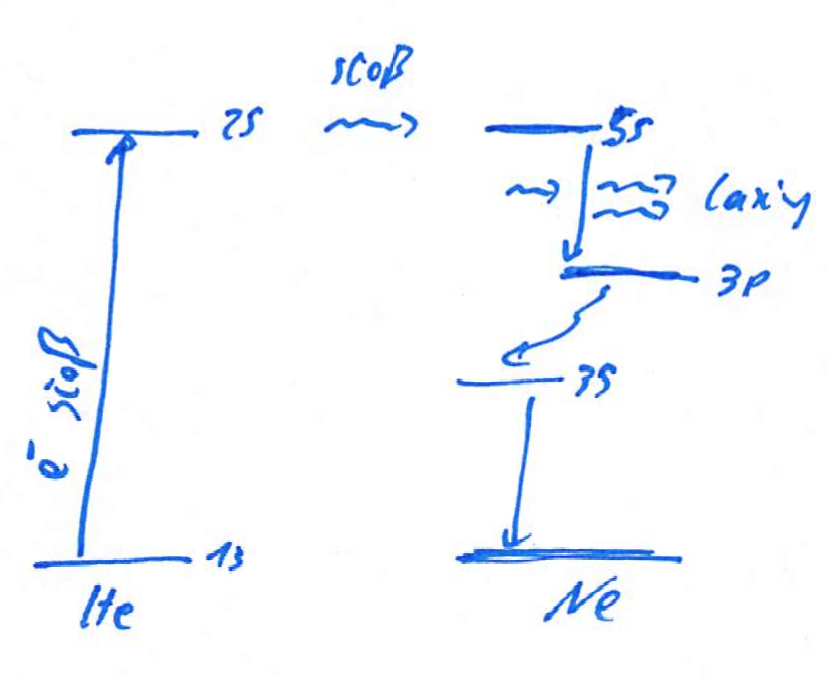
\includegraphics[width=\textwidth]{\currfiledir png/hene.png}
    \caption{Die relevanten Zustände des He-Ne-Lasers.}
    \label{fig:7_hene_laser}
\end{marginfigure}

\section{Linienbreiten}

Bisher haben wir nur die Lage der Linien im Atomspektrum diskutiert, wobei wir immer davon ausgegangen sind, dass sie deltaförmig sind. Das ist nicht der Fall. Wenn man hochauflösende Spektroskopie betreibt, beobachtet man eine Linienbreite, die größer ist als die experimentelle Auflösung. Drei Ursachen werden hier diskutiert.

\subsection{Natürliche Linienbreite} 

Selbst bei einem idealen Atom muss aufgrund der Energie-Zeit-Unschärfe (oder der Fourier-Transformation) ein Zusammenhang zwischen der Lebensdauer des angeregten Zustands und der spektralen Breite des Übergangs bestehen. Je länger ich eine Frequenz messen kann, desto genauer kann ich sie bestimmen. Die resultierende Linienbreite wird als 'natürlich' bezeichnet, da sie die fundamentale Grenze darstellt. Für sie gilt
\begin{equation}
    \delta \nu_\text{nat} = \frac{1}{2\pi \, \tau}
\end{equation}
mit der Lebensdauer $\tau$ des angeregten Zustands. Für die Natrium-D-Linie aus dem Zustand 3D$_{1/2}$ ergibt sich bei einer Lebensdauer von $\tau = 16$~ns eine Linienbreite von $\delta \nu_\text{nat} = 10$~MHz.

\paragraph{Nebenbemerkung} Wenn Sie es merkwürdig finden, dass hier die Lebensdauer des Zustands eingeht, während das Atom nur darauf wartet, dass es endlich emittiert, dann liegt das an all den Dingen, die wir weggelassen haben. Lesen Sie dann über  'Rabi-Oszillationen' und stellen fest, dass Quantensprünge manchmal doch nicht instantan sind.


\subsection{Doppler-Verbreiterung}


Bewegt sich eine Atom mit der Geschwindigkeit  $v$ in Strahlrichtung, so ändert sich seine Absorptions-Frequenz aufgrund der Doppler-Verschiebung um $\Delta \nu$.
\begin{equation}
	\Delta \nu = \frac{v}{c_0} \, \nu_0
\end{equation}
mit der Ruhe-Frequenz $\nu_0$. Die Geschwindigkeit kommt  aus der  Maxwell-Boltzmann-Geschwindigkeitsverteilung $\mathcal{P}(v)$
\begin{equation}
	\mathcal{P}(v) = \sqrt{\frac{m}{2 \pi k_B T}} \, \exp \left (
	- \frac{m v^2}{2  k_B T}	
	\right) \quad .
\end{equation}
mit der Masse $m$ des Atoms.
Insgesamt ergibt sich damit eine gaußförmige  Linie der Halbwertsbreite 
\begin{equation}
	 \delta \nu_{doppler} = \nu_0 \, \sqrt{\frac{8 k_B T \ln 2} {m c^2}} \quad .
\end{equation}
Für die Natrum-D-Linie ergibt sich  $\delta \nu_{doppler} = 1 \, 700$~MHz. Sie übertrifft damit die natürliche Linienbreite bei weitem.

\subsection{Stoß-Verbreiterung}

Stößt ein Atom mit einem anderen zusammen, während es sich im angeregten Zustand befindet, so wird die Lebensdauer des angeregten Zustandes effektiv verkürzt, $\tau$ wird kürzer und damit wie oben $\delta \nu$ breiter. Die mittlere Zeit $\delta t$ zwischen den Stößen kann aus der mittleren freien Weglänge $l$ eines Gases der mittleren Geschwindigkeit $v$ abgeschätzt werden (\cite{Demtroeder_laser}) % eq. 3.52, demtröder laser spectrsocpy I
\begin{equation}
    \Delta t = \frac{l}{v} = \frac{1}{n \sigma} \, \sqrt{ \frac{\pi \mu}{8 k_B T}} \quad .
\end{equation}
Dabei ist $n$ die Teilchendichte (proportional zum Druck\sidenote{daher manchmal auch Druckverbreiterung genannt} $p$) des Stoßpartners, $\sigma$ ein Streuquerschnitt, der die effektive Größe des Atoms beschreibt, und $\mu$ die reduzierte  Masse aus Atom und (ggf. anderem) Stoßpartner. Für die Liniebreite gilt dann wieder
\begin{equation}
    \delta \nu_\text{stoss} = \frac{1}{2\pi \, \Delta t} = p \, \sigma \sqrt{ \frac{8}{\pi \mu k_B T}} \quad .
\end{equation}
Bei spektroskopischen Experimenten kann man hier den Druck und damit die Teilchendichte $n$ verringern und diesen Verbreitungsmechanismus ausschalten. 


% XXX Rubidium Experiment ???

\section{Röntgenstrahlung}

In den einleitenden Kapiteln wurde bereits kurz über Röntgenstrahlung gesprochen. Röntgenstrahlung ist wie das sichtbare Licht eine elektromagnetische Welle. Der Unterschied besteht darin, dass die Energie pro Photon wesentlich höher ist. In diesem Kapitel wurde bisher nur ein Valenzelektron angeregt. In Abbildung \ref{fig:6_PSE_states} des letzten Kapitels sieht man jedoch, dass die tiefer gelegenen gebundenen Elektronen deutlich stärker gebunden sind als das Valenzelektron und ihre Übergänge daher mit sehr energiereichen Photonen verbunden sind. Wir betrachten nun also die Spektroskopie der inneren Elektronen.

\subsection{Bremsstrahlung}


\begin{marginfigure}
    \inputtikz{\currfiledir bremsstrahlung} 
    \caption{Brems-Spektrum einer Wolfram-Anode bei $U= 15, 25, 35, 50$~kV. Daten von \cite{Gilfrich68}.}
    \label{fig:7_bremsstrahlung}
\end{marginfigure}

Bevor wir zu diesem Punkt kommen, müssen wir kurz auf die Bremsstrahlung eingehen. Darunter versteht man ein breites Kontinuum im Röntgenspektrum,  das nicht vom Kathodenmaterial abhängt. Die durch die Spannung $U$ beschleunigten Elektronen werden an den Kernen des Kathodenmaterials abgelenkt, ohne dass die Kerne oder die Elektronen des Kathodenmaterials Energie aufnehmen. Ablenkung bedeutet Beschleunigung, und die beschleunigten Elektronen sind die Quelle  elektromagnetischer Strahlung.  Das Kontiunium hat eine maximale Frequenz bzw. eine minimale Wellenlänge, die von der Beschleunigungsspannung $U$ abhängt: Maximal kann die gesamte Energie $e \, U$ auf ein Photon übertragen werden.
\begin{equation}
    h \nu_\text{grenz} = e \, U \quad \text{oder} \quad
    \lambda_\text{grenz} = \frac{h c}{e U} \quad .
\end{equation}
Beschleunigungsspannungen im Bereich von einigen 10~kV ergeben Wellenlängen von 0.1--1~nm (und natürlich Photonenenergien von einigen 10~keV).

Das Spektrum der Bremsstrahlung ist in einem einfachen Modell linear in $\nu$, also 
\begin{equation}
    I(\nu) d\nu \propto \nu_\text{grenz} - \nu \quad \text{für} \quad  \nu < \nu_\text{grenz} \quad .
\end{equation}
Nach Umrechnung auf eine Wellenlängenskala ergibt sich
\begin{equation}
    I(\lambda) d\lambda \propto \left( \frac{\lambda}{\lambda_\text{grenz}} - 1 \right) \frac{1}{\lambda^2} 
    \quad \text{für} \quad  \lambda > \lambda_\text{grenz} \quad .
\end{equation}




\subsection{Charakteristisches Linienspektrum}

Experimentell findet man neben dem Kontinuum der Bremsstrahlung eine für das Kathodenmaterial charakteristische Abfolge von scharfen Linien. Hier wird ein inneres Elektron des Kathodenmaterials aus dem Atom herausgeschlagen. Eines der verbleibenden, energetisch höheren Elektronen fällt unter Aussendung eines Röntgenphotons in diese Lücke zurück. Die Lage der Linien hängt also von zwei Zuständen ab: dem des herausgeschlagenen Elektrons und dem des auffüllenden Elektrons.

\begin{marginfigure}
    \inputtikz{\currfiledir linienspektrum} 
    \caption{Linien-Spektrum einer Wolfram-Anode bei 45 kV mit den charakteristischen L-Linien. Daten von \cite{Gilfrich68}.}
    \label{fig:7_linienspektrum}
\end{marginfigure}


Ein einfaches Modell, das Moseley-Gesetz, ignoriert alle Details auf atomarer Ebene und geht einfach von einem wasserstoffähnlichen System aus. In diesem Fall wird die Energie eines Zustands nur durch seine Hauptquantenzahl $n$ beschrieben. Die Energie des emittierten Röntgenphotons ist dann 
\begin{equation}
    h \nu = (Z - S_n)^2 \, R_H \, hc \, \left(  \frac{1}{n^2} - \frac{1}{m^2} \right) \quad .
\end{equation}
Dabei ist $n$ die Quantenzahl des herausgeschlagenen Elektrons und $m$ die des auffüllenden. Der Parameter $S_n$ korrigiert die Kernladung $Z$ um die weiter innen liegenden Elektronen und ist daher von $n$ abhängig. Für $n=1$ ist $S \approx 1$, für $n=2$ ist $S \approx 7,8$.
Wie bei den Schalen der Mehrelektronenatome werden die Linien(gruppen) entsprechend der Quantenzahl $n = 1, 2, 3$ mit den Buchstaben K, L, M bezeichnet. Die Quantenzahl $m$ wird in ihrem Abstand von $n$ durch griechische Buchstaben kodiert: $\alpha, \beta, \gamma$ bedeutet also $m=n + 1,2,3$. Die Linie K$_\alpha$ entspricht einem Übergang von $m=2$ nach $n=1$, die Linie L$_\gamma$ einem Übergang von $m=5$ nach $n=2$.

\subsection{Absorption}

Absorptionsspektren können auch mit Röntgenstrahlen gemessen werden. Wie immer nimmt die transmittierte Leistung $P$ exponentiell mit der Dicke des Materials ab.
\begin{equation}
    P(x)  = P_0 e^{- \alpha x} = P_0 \, e^{- n \sigma  x}
\end{equation}
mit dem Absorptionskoeffizienten $\alpha$. Dieser ist das Produkt aus der Teilchenzahldichte $n$ und dem Absorptionsquerschnitts $\sigma$ ab. Der Absorptionsquerschnitts beschreibt dem Effekt jedes einzelnen Atoms auf die Röntgenstrahlung.

Drei Effekte tragen zur Absorption von Röntgenphotonen bei
\begin{description}
    \item[Photoeffekt] Das Röntgenphoton wird vom Atom absorbiert. Dabei wird ein stark gebundenes Elektron ionisiert und auch das Atom erhält  kinetische Energie.
    \item[Compton-Effekt] Das Röntgenphoton stößt mit einem fast freien Elektron einer der äußeren Schalen des Atoms. Dabei übernimmt das Elektron kinetische Energie und die Wellenlänge des Röntgenphotons ändert sich.
    \item[Paarerzeugung] Bei ausreichend hohen Energien des Röntgenphotons ($E > 1$MeV) kann ein Elektron-Positron-Paar erzeugt werden. Hier wird Energie in Materie umgewandelt! Die restliche Energie geht in die kinetische Energie der neuen Teilchen.
\end{description}

Solange die Energie noch nicht für Paarerzeugung ausreicht, findet man
\begin{equation}
    \sigma \approx C \, Z^4 \, \lambda^3 \quad .
\end{equation}
Die Absorption nimmt also mit der Kernladungszahl und der Wellenlänge stark zu. Die Konstante $C$ hängt von der Quantenzahl $n$ bzw. der beteiligten Schale ab: Mit zunehmender Wellenlänge reicht die Energie des Röntgenphotons irgendwann nicht mehr aus, um Elektronen einer Schale zu ionisieren. Die K-Kante im Absorptionsspektrum fällt daher mit der Grenze der K-Serie im Emissionsspektrum zusammen.


\newpage

\section{Zusammenfassung}

\textit{Schreiben Sie hier ihre persönliche Zusammenfassung des Kapitels auf. Konzentrieren Sie sich auf die wichtigsten Aspekte.}

\vspace*{10cm}


%--------------------
\printbibliography[segment=\therefsegment,heading=subbibliography]
